\documentclass{beamer}
\usepackage[utf8]{inputenc}
\usetheme{Madrid}
\usepackage{tikz}
\usetikzlibrary {arrows.meta}
\usepackage{wrapfig}

%------------------------------------------------------------
%This block of code defines the information to appear in the
%Title page
\title[Rust Macros]
{RUST MACROS}

\author
{
Sebastian Vișan\\
}

\institute[]
{
  University of Helsinki\\
  Faculty of Science\\
  Master of Computer Science
}

\date % (optional)
{6 Nov 2025}

\begin{document}

%The next statement creates the title page.
\frame{\titlepage}

% In many ways macros are like functions, but because they have more power/they do more stuff, they are harder to read or write
% There are many fine details that are easy to mix up, the rust book alreaady does a great job at teaching these
% The goal of the presentation is to be accessible to people who have never dealt with macros
% Compromise: explain the main ideas of macros at a high level, show a couple of examples that I found relevant
\begin{frame}
\frametitle{Challenges}
Metaprogramming is confusing...
\\~\\

\begin{itemize}
    \item<2-> to implement
    \item<3-> to discuss
    \item<4-> to follow
\end{itemize}
\end{frame}

% Talk about compilation vs run time
% Half of the battle is getting your code to compile, logic errors result in compilation errors
% Macros are useful for dealing with repetitive code

\begin{frame}[t]{What is a \textit{Macro}?}

\pause

A function that outputs code

\pause

\vspace{1cm}

\begin{center}
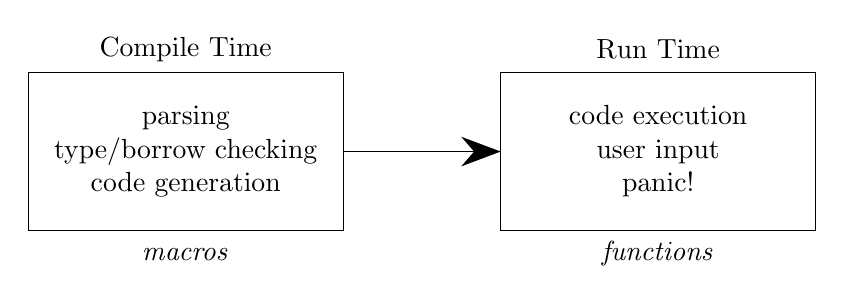
\begin{tikzpicture}

\draw (10,12) rectangle (14, 14);
\draw (16,12) rectangle (20,14);
\draw [-{Stealth[length=5mm]}] (14, 13) -- (16, 13);
\node at (12,14.3) {Compile Time};
\node at (18,14.3) {Run Time};
\node at (12,13) {\begin{tabular}{c} parsing\\type/borrow checking\\code generation \end{tabular}};
\node at (18,13) {\begin{tabular}{c} code execution\\user input\\panic! \end{tabular}};
\pause
\node at (12,11.7) {\begin{tabular}{c} \textit{macros} \end{tabular}};
\node at (18,11.7) {\begin{tabular}{c} \textit{functions} \end{tabular}};

\end{tikzpicture}
\end{center}
    
\end{frame}

\begin{frame}{Types of Macros}


\begin{block}{\textbf{Declarative}}
     \texttt{macro\_rules!}
\end{block}
\begin{block}{\textbf{Procedural}}
    \begin{itemize}
        \item \textbf{Derive} \\
        \texttt{\#[proc\_macro\_derive()]}
        \item \textbf{Attribute-Like} \\
        \texttt{\#[proc\_macro\_attribute]}
        \item \textbf{Function-Like} \\
        \texttt{\#[proc\_macro]}
    \end{itemize}
\end{block}

\end{frame}

%---------------------------------------------------------

% How could we implement println as a function?
% Variable number of arguments -> Maybe list of arguments (not the same type though)
% Formatting errors detected at runtime :(
\begin{frame}{Declarative Macros}
Most common type of macro. \\
Work with well defined structure. \\
\pause
Some familiar examples:

\centering
    \includegraphics[width = 12cm]{declarative.png}

\pause
Most of these are implemented directly by the compiler.

\end{frame}

\begin{frame}{Declarative Macros}

\begin{tikzpicture}
  \node (A) at (0,0)     {\includegraphics[width=12cm]{vec_macro.png}};
  \pause
  \node (B) at (0,-4.5)  {\includegraphics[width=12cm]{vec_expanded.png}};
  \node (C) at (-1, -1.4) [left]{macro expansion};
  \draw[-{Stealth[length=5mm]}] ([xshift=-4cm]A.south) -- ([xshift=-4cm]B.north);
  \pause
  \node (D) at (7, -5.5) {\includegraphics[width = 12cm]{vec_alternatives.png}};
\end{tikzpicture}

\end{frame}

%---------------------------------------------------------

\begin{frame}[t]{Procedural Derive Macros}

Used on enums and structs. \\
Provide automated trait implementations.

\includegraphics<2>[width=10cm]{derive_enum.png}
\includegraphics<3>[width=11cm]{derive_struct.png}

\pause
\pause
The \texttt{i32} field also needs to implement the traits. 

\end{frame}

\begin{frame}[t]{Procedural Derive Macros}

We can use the \textbf{cargo expand} crate to look at the generated code after the macro expansion:

\includegraphics[width = 12cm]{derive_struct_expanded.png}

Notice the check that \texttt{i32} implements the \texttt{Clone} trait.

\end{frame}

\begin{frame}[t]{Procedural Attribute-Like Macros}

\begin{minipage}{0.5\textwidth}
Very similar to custom derive macros, \\
but also work for other items than \\
structs and enums. 
\end{minipage}
\hfill
\begin{minipage}{0.45\textwidth}
\includegraphics[width=7cm, left]{attribute_route.png}
\end{minipage}

\pause

\\~\\
Other familiar attributes:

\includegraphics[width=11cm]{attribute_examples.png}

\end{frame}

\begin{frame}[t]{Procedural Function-Like Macros}

Invocation looks like that of declarative macros. \\
They work on arbitrary token streams as opposed to defined structured patterns.

\includegraphics[width=11cm]{proc_sql.png}

\pause

Custom syntax allows us to write embedded DSLs (domain specific languages). \\
These macros are very powerful, but less readable.

\end{frame}

%---------------------------------------------------------
% We don't want to repeat ourselves, we see the pattern and want to write it only once
% We could write a function using closures, but then we have to handle references and mutating variables
% We just want to take the line of code that we care about and insert code before and after it => Macro
\begin{frame}[t]{Example1 - timed!}

Problem: benchmark how much time a specific block of code takes to run.

\pause

Solution: measure the time before and after, then subtract.

\pause

\includegraphics[width=11cm]{timed_sol.png}

\pause

Problem: boilerplate \\
Could we write a function for this? 
\pause 
No, can't pass code block as argument.

\end{frame}

\begin{frame}{Example1 - timed!}

Declarative macro that expands our code block into a timed version:

\includegraphics[width=12cm]{timed_macro.png}

\end{frame}

\begin{frame}[t]{Example1 - timed!}

\includegraphics[width=10cm]{timed_example1.png}
\pause
\includegraphics[width=12cm, trim=1cm 0 0 2cm]{timed_example1_expanded.png}

\end{frame}

\begin{frame}{Example1 - timed!}

\includegraphics[width=8cm]{timed_example2.png}

\end{frame}

%---------------------------------------------------------

\begin{frame}[t]{Example2 - comp!}

What we'll build: simplified Python List Comprehension

\includegraphics[width=8.5cm, trim=-7cm 0 0 0cm]{comp_python.png}

\pause

How would we write this in Rust?

\includegraphics[width=10cm, trim=-2cm 0 0 0cm]{comp_rust_iter.png}

\pause

Architecture: \textbf{syn} and \textbf{quote} crates

\begin{center}
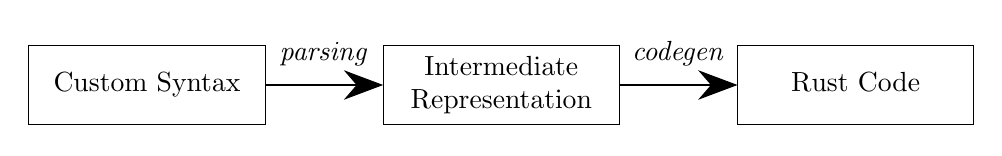
\begin{tikzpicture}

\draw (-1.5,0) rectangle (1.5, 1);
\draw (-6,0) rectangle (-3, 1);
\draw (3,0) rectangle (6,1);
\draw [-{Stealth[length=5mm]}] (-3, 0.5) -- (-1.5, 0.5);
\draw [-{Stealth[length=5mm]}] (1.5, 0.5) -- (3, 0.5);
\node at (-4.5,0.5) {\begin{tabular}{c} Custom Syntax \end{tabular}};
\node at (-2.25,0.9) {\begin{tabular}{c} \textit{parsing} \end{tabular}};
\node at (0,0.5) {\begin{tabular}{c} Intermediate\\Representation \end{tabular}};
\node at (2.25,0.9) {\begin{tabular}{c} \textit{codegen} \end{tabular}};
\node at (4.5,0.5) {\begin{tabular}{c} Rust Code \end{tabular}};

\end{tikzpicture}
\end{center}

\end{frame}

\begin{frame}[t]{Example2 - comp!}

Intermediate Representation: \\
Using \texttt{Expr} and \texttt{Pat} types from \texttt{syn}

\includegraphics[width=10cm]{comp_type.png}

Parse \texttt{[x * w for x <- xs]} into:\\
\texttt{Comp \{mapping = x * 2, pattern: x, sequence: xs\}}

\end{frame}

\begin{frame}[t]{Example2 - comp!}

Parsing using the syn crate:

\includegraphics[width=10cm]{comp_parse.png}

\end{frame}

\begin{frame}[t]{Example2 - comp!}

Codegen using the quote crate:

\includegraphics[width=12cm]{comp_proc_macro.png}

\end{frame}

\begin{frame}{Example2 - comp!}

Results:

\includegraphics[width=12cm]{comp_results.png}

\pause 

Adding custom syntax would be very confusing in a real world project,\\
but macros can be very fun to write and experiment with!

\end{frame}

%---------------------------------------------------------

\begin{frame}
\frametitle{Resources}

\begin{itemize}
    \item \textbf{Code for Examples} \\ https://github.com/VSebastian8/rust-macros
    \item \textbf{The Rust Programming Language} https://doc.rust-lang.org/book/ch20-05-macros.html
    \item \textbf{The Little Book of Rust Macros} https://lukaswirth.dev/tlborm/decl-macros.html
    \item \textbf{Comprehending Proc Macros} https://www.youtube.com/watch?v=SMCRQj9Hbx8
\end{itemize}

\end{frame}


\end{document}